\documentclass[aspectratio=169]{beamer}

% ---------- THEME & LOOK ----------
\usetheme{Madrid}
\usecolortheme{seahorse}
\usefonttheme{professionalfonts}
\setbeamertemplate{navigation symbols}{}
\setbeamercovered{transparent}
\setbeamertemplate{itemize items}[circle]
\setbeamertemplate{enumerate items}[default]
\setlength{\parskip}{0.25em}

% ---------- COLORS ----------
\usepackage{xcolor}
\definecolor{accent}{RGB}{0,92,184}
\definecolor{soft}{RGB}{233,244,255}
\setbeamercolor{structure}{fg=accent}
\setbeamercolor{title}{fg=white,bg=accent}
\setbeamercolor{frametitle}{fg=accent}
\setbeamercolor{block title}{bg=accent!10,fg=accent}
\setbeamercolor{block body}{bg=soft}

% ---------- PACKAGES ----------
\usepackage{booktabs}
\usepackage{amsmath, amssymb}
\usepackage{array}
\usepackage{hyperref}
\hypersetup{colorlinks=true,linkcolor=accent,urlcolor=accent}

% ---------- PLACEHOLDER BOX ----------
\newcommand{\placeholderbox}[2][0.82\linewidth]{%
  \begin{center}
    \fbox{\begin{minipage}[c][0.46\textheight][c]{#1}
      \centering \vspace{0.25em}
      \textbf{#2}\\[0.6em]
      \emph{Insert figure/table here later.}
    \end{minipage}}
  \end{center}
}

% ---------- TITLE ----------
\title{\textbf{Human Capital Theory: Applications to Education and Training}}
\subtitle{{\large ECON 300 - Labour Economics}}
\author{Muhebullah Karimzada}
\date{Winter 2026}

\begin{document}

% ============================================================
% TITLE
% ============================================================
\begin{frame}[plain]
  \titlepage
\end{frame}

% ============================================================
\section{Orientation}
% ============================================================

\begin{frame}{Learning Objectives}
\transfade
\begin{itemize}[<+->]
  \item Discuss how the decision to invest in human capital --- schooling or on-the-job training --- can be analyzed as a standard \textbf{investment decision}.
  \item Explain why the most expensive part of human capital investment is often the \textbf{opportunity cost of time}.
  \item Explain why comparing wages of more- and less-educated workers can be misleading because of:
  \begin{itemize}[<+->]
    \item \textbf{ability bias}, and
    \item the use of education as a \textbf{signal} in the labour market.
  \end{itemize}
  \item Describe why the return to education is large and has increased over time in Canada.
  \item Discuss when workers or employers should pay for training programs.
\end{itemize}
\end{frame}

\begin{frame}{Main Questions I}
\transfade
\begin{itemize}[<+->]
  \item Why are more-educated workers generally paid more than less-educated workers?
  \item What factors determine the market rate of return to education?
  \item If education is such a worthwhile investment, why does not everyone pursue very high levels of education?
  \item Are more-educated people paid more because education raises productivity, or because education reveals greater inherent productivity?
  \item What are \textbf{signalling} and \textbf{screening} in labour markets?
\end{itemize}
\end{frame}

\begin{frame}{Main Questions II}
\transfade
\begin{itemize}[<+->]
  \item How might education serve as a signal?
  \item If education is mainly a screening device, why might the \textbf{private} and \textbf{social} returns to education differ?
  \item Should the government subsidize early childhood learning?
  \item Are government-funded training programs worth the money?
\end{itemize}

\begin{block}{Big Idea}
Human capital theory connects labour economics with investment theory: individuals compare present costs with future benefits.
\end{block}
\end{frame}

% ============================================================
\section{Human Capital Theory}
% ============================================================

\begin{frame}{Human Capital Theory}
\transfade
\begin{block}{Definition}
\textbf{Human capital} refers to the stock of skills, knowledge, abilities, and training that increases a person's productivity and earning power.
\end{block}
\begin{itemize}[<+->]
  \item Investments are made to improve productivity and earnings.
  \item Costs are incurred today with the expectation of future benefits.
  \item Rational investment requires that expected benefits exceed expected costs.
\end{itemize}

\begin{exampleblock}{Example}
A student who spends four years in university gives up current earnings but expects higher wages for decades afterward.
\end{exampleblock}
\end{frame}

\begin{frame}{Types of Costs and Benefits}
\transfade
\begin{itemize}[<+->]
  \item \textbf{Opportunity cost:} forgone income while studying or training.
  \item \textbf{Private costs and benefits:} those borne or enjoyed directly by the individual.
  \item \textbf{Social costs and benefits:} those affecting society as a whole.
  \item \textbf{Real costs:} actual use of resources such as teachers, classrooms, and books.
  \item \textbf{Transfer costs:} payments that reallocate resources, such as taxes or subsidies.
\end{itemize}

\begin{block}{Key Point}
The largest cost of schooling is often not tuition, but the earnings the student gives up by not working.
\end{block}
\end{frame}

% ============================================================
\section{Private Investment in Education}
% ============================================================

\begin{frame}{Private Investment in Education}
\centering

\includegraphics[width=0.7\linewidth]{F1}
\end{frame}

\begin{frame}{Understanding Alternative Income Streams}
\transfade
\begin{itemize}[<+->]
  \item Education usually causes earnings to be \textbf{lower early in life} because the student is in school.
  \item Later, education may produce \textbf{higher annual earnings}.
  \item The investment decision depends on whether the later gains outweigh the earlier losses.
\end{itemize}

\begin{block}{Interpretation}
Human capital investment changes the entire \textbf{age-earnings profile}, not just current income.
\end{block}
\end{frame}

\begin{frame}{Age-Earnings Profiles}
\transfade
\begin{itemize}[<+->]
  \item Earnings usually increase with age and experience.
  \item The increase occurs at a decreasing rate.
  \item Age-earnings profiles are typically higher for workers with more education.
\end{itemize}

\begin{exampleblock}{Example}
A university graduate may earn less than a high school graduate at age 20, but more by age 30 or 35.
\end{exampleblock}
\end{frame}

\begin{frame}{Optimal Human Capital Investment}
\transfade
\begin{block}{Simplifying Assumptions}
\begin{itemize}[<+->]
  \item Education provides no direct utility or disutility.
  \item Hours of work are fixed.
  \item Income streams associated with education are known.
  \item Individuals can borrow and lend at the real interest rate.
\end{itemize}
\end{block}

\begin{block}{Purpose}
These assumptions make the schooling decision a standard \textbf{present value maximization problem}.
\end{block}
\end{frame}

\begin{frame}{Formal Analysis of Benefits}
\transfade
Consider an 18-year-old high school graduate deciding whether to work or go to college.

The present value of a constant income stream over working years can be written as:
\[
PV = \sum_{t=18}^{T} \frac{Y}{(1+r)^t}
\]

where:
\begin{itemize}[<+->]
  \item \(Y\) = annual income,
  \item \(r\) = market interest rate (discount rate),
  \item \(T\) = retirement age.
\end{itemize}

\begin{block}{Interpretation}
The higher the discount rate, the less valuable future earnings become today.
\end{block}
\end{frame}

\begin{frame}{Marginal Costs and Benefits of Schooling}
\transfade
\begin{itemize}[<+->]
  \item The decision to take \textbf{one more year of schooling} depends on:
  \begin{itemize}[<+->]
    \item \textbf{Marginal cost} of the extra year
    \item \textbf{Marginal benefit} of the extra year
  \end{itemize}
  \item The return to schooling can also be summarized by the \textbf{internal rate of return}.
\end{itemize}

\begin{block}{Definition}
The \textbf{internal rate of return} is the discount rate that makes the present value of benefits equal to the present value of costs.
\end{block}
\end{frame}

\begin{frame}{Marginal Cost of One More Year of Education}
\transfade
The cost of one more year of post-secondary education can be written as:
\[
MC = Y + D
\]
where:
\begin{itemize}[<+->]
  \item \(Y\) = forgone income while attending school,
  \item \(D\) = direct cost of one more year of school.
\end{itemize}

\begin{exampleblock}{Example}
If a student gives up \$35,000 in earnings and pays \$7,000 in tuition and books, the marginal cost is \$42,000.
\end{exampleblock}
\end{frame}

\begin{frame}{Marginal Benefit of One More Year of Education}
\transfade
The benefit of one more year of schooling is the increase in annual income:
\[
MB = \Delta Y
\]

The optimal quantity of education is achieved when:
\[
MB = MC
\]
or equivalently:
\[
i = r
\]

where:
\begin{itemize}[<+->]
  \item \(i\) = internal rate of return,
  \item \(r\) = market interest rate.
\end{itemize}
\end{frame}

\begin{frame}{Figure 9.2: Decision Rule for Optimal Human Capital Investment}
\centering

\includegraphics[width=0.4\linewidth]{F2}
\end{frame}

\begin{frame}{Decision Rule for Education}
\transfade
To maximize the net present value of lifetime earnings, increase education until:
\begin{itemize}[<+->]
  \item the present value of benefits of an additional year equals the present value of costs, or
  \item \(i = r\).
\end{itemize}

\begin{block}{Economic Intuition}
\begin{itemize}[<+->]
  \item If \(i > r\), schooling yields a better return than financial investment.
  \item If \(i < r\), the individual should stop investing in schooling.
\end{itemize}
\end{block}
\end{frame}

\begin{frame}{Implications of the Theory}
\transfade
\begin{itemize}[<+->]
  \item Investment in education should occur early in life because the benefits last longer.
  \item Individuals expecting interruptions in labour force participation may invest less.
  \item A progressive tax system can reduce private incentives to invest in education because it reduces after-tax returns.
\end{itemize}

\begin{exampleblock}{Example}
Someone planning only a short working career has fewer years to recoup the cost of schooling.
\end{exampleblock}
\end{frame}

\begin{frame}{Factors Influencing Education}
\transfade
\begin{itemize}[<+->]
  \item \textbf{Income tax:} greater progressivity lowers the after-tax return to education.
  \item \textbf{Student loans:} reduce borrowing constraints and make schooling more accessible.
  \item \textbf{Government support:} subsidies can increase educational attainment and productivity.
\end{itemize}

\begin{block}{Key Point}
Policies affect schooling both by changing the \textbf{cost of education} and by changing the \textbf{return to education}.
\end{block}
\end{frame}

\begin{frame}{Worked Example: Computing the Return to Education}
\transfade
Mary is an 18-year-old high school graduate who can earn \$30{,}000 immediately.
The market interest rate is \(5\%\), and she plans to work until age 65.
\begin{itemize}[<+->]
  \item Without further education, her annual earnings are \$30{,}000.
  \item With one more year of schooling, her annual earnings rise to \$33{,}000.
\end{itemize}

\begin{block}{Question}
Should Mary invest in one additional year of education?
\end{block}
\end{frame}

\begin{frame}{Approximating Present Value}
\transfade
A perpetual stream of income \(Y\) can be approximated by:
\[
PV \approx \frac{Y}{r}
\]

This approximation is useful when comparing long-run income streams.

\begin{itemize}[<+->]
  \item If \(Y = 30{,}000\) and \(r = 0.05\), then
  \[
  PV \approx \frac{30{,}000}{0.05} = 600{,}000
  \]
  \item If income rises to \(33{,}000\),
  \[
  PV \approx \frac{33{,}000}{0.05} = 660{,}000
  \]
\end{itemize}
\end{frame}

\begin{frame}{Mary's Return to Education}
\transfade
The increase in present value from one more year of schooling is approximately:
\[
660{,}000 - 600{,}000 = 60{,}000
\]

The textbook example reports that the extra year of schooling raises the present value of future income by about \$23{,}943 using a finite working-life horizon.

The internal rate of return can be approximated by:
\[
i = \frac{\Delta Y}{Y + D}
\]

\begin{itemize}[<+->]
  \item If \(D=0\):
  \[
  i = \frac{3000}{30{,}000}=10\%
  \]
  \item If \(D=3000\):
  \[
  i = \frac{3000}{33{,}000}\approx 9\%
  \]
\end{itemize}
\end{frame}

\begin{frame}{Interpreting the Worked Example}
\transfade
\begin{itemize}[<+->]
  \item If the internal rate of return exceeds the market interest rate, schooling is a worthwhile investment.
  \item Mary should invest because:
  \[
  10\% > 5\%
  \]
  \item Direct costs would need to become much larger before the investment would stop being worthwhile.
\end{itemize}

\begin{exampleblock}{Interpretation}
Education is attractive here because the earnings gain is large relative to both forgone income and direct costs.
\end{exampleblock}
\end{frame}

% ============================================================
\section{Education as a Filter}
% ============================================================

\begin{frame}{Education as a Filter}
\transfade
\begin{block}{Definition}
Education may act as a \textbf{filter}, \textbf{signal}, or \textbf{screening device} if it helps employers identify worker productivity rather than directly increasing productivity.
\end{block}
\begin{itemize}[<+->]
  \item Employers may offer higher wages to educated workers because they believe education signals higher productivity.
  \item In this view, education helps sort workers rather than necessarily making them more productive.
\end{itemize}
\end{frame}

\begin{frame}{Figure 9.3: Offered Wage and Signalling Cost Schedules}
\centering
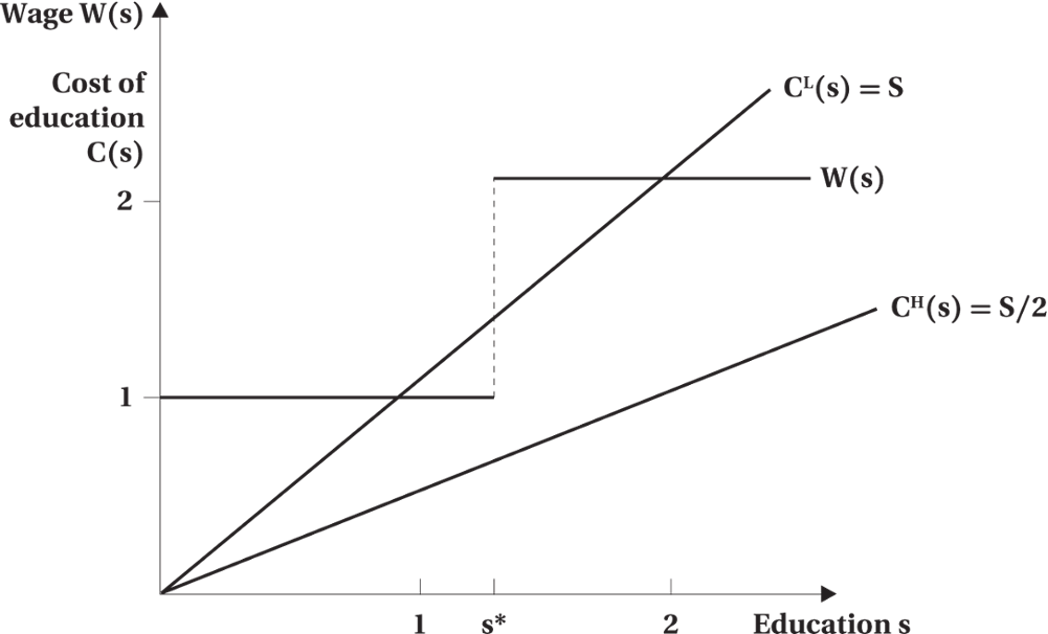
\includegraphics[width=0.7\linewidth]{F3}
\end{frame}

\begin{frame}{Interpreting Signalling and Screening}
\transfade
\begin{itemize}[<+->]
  \item \textbf{Signalling:} workers obtain education to signal desirable traits such as ability, persistence, or discipline.
  \item \textbf{Screening:} firms use education to sort applicants.
  \item If signalling is very important, the \textbf{private return} to education may exceed the \textbf{social return}.
\end{itemize}

\begin{exampleblock}{Example}
An employer may interpret a university degree as evidence that the applicant is more productive, even if the job uses only part of what was learned.
\end{exampleblock}
\end{frame}

% ============================================================
\section{Empirical Evidence: Education and Earnings}
% ============================================================

\begin{frame}{Empirical Evidence: Education and Earnings}
\transfade
\begin{itemize}[<+->]
  \item Earnings increase with age and experience.
  \item The increase is usually most rapid up to middle age.
  \item The earnings gap between education groups tends to widen over the life cycle.
\end{itemize}

\begin{block}{Interpretation}
This pattern is consistent with human capital accumulation and higher long-run rewards to education.
\end{block}
\end{frame}

\begin{frame}{Figure 9.4: Earnings by Age and Education}
\centering
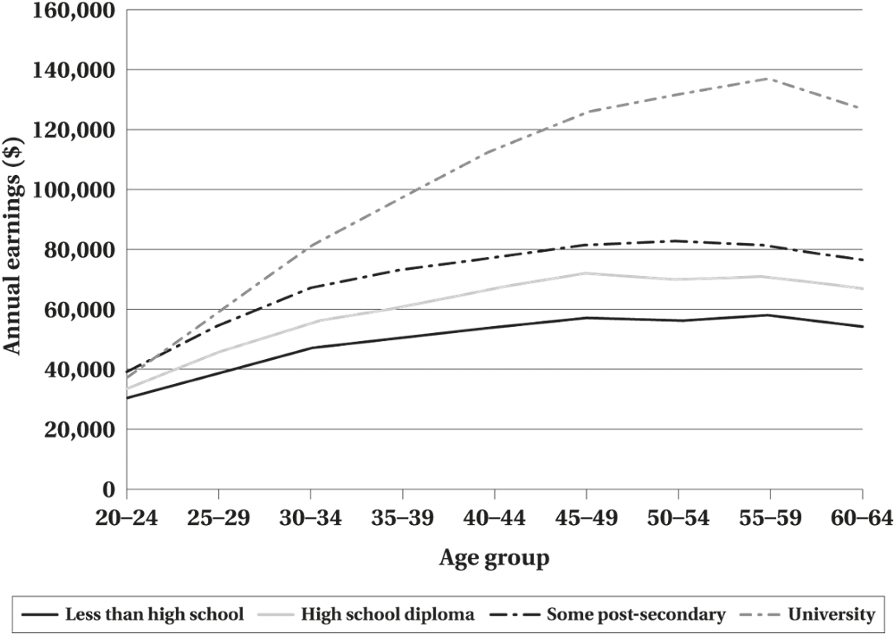
\includegraphics[width=0.6\linewidth]{F4}
\end{frame}

\begin{frame}{Table 9.1: Estimates of the Private Returns to Schooling in Canada}
\centering
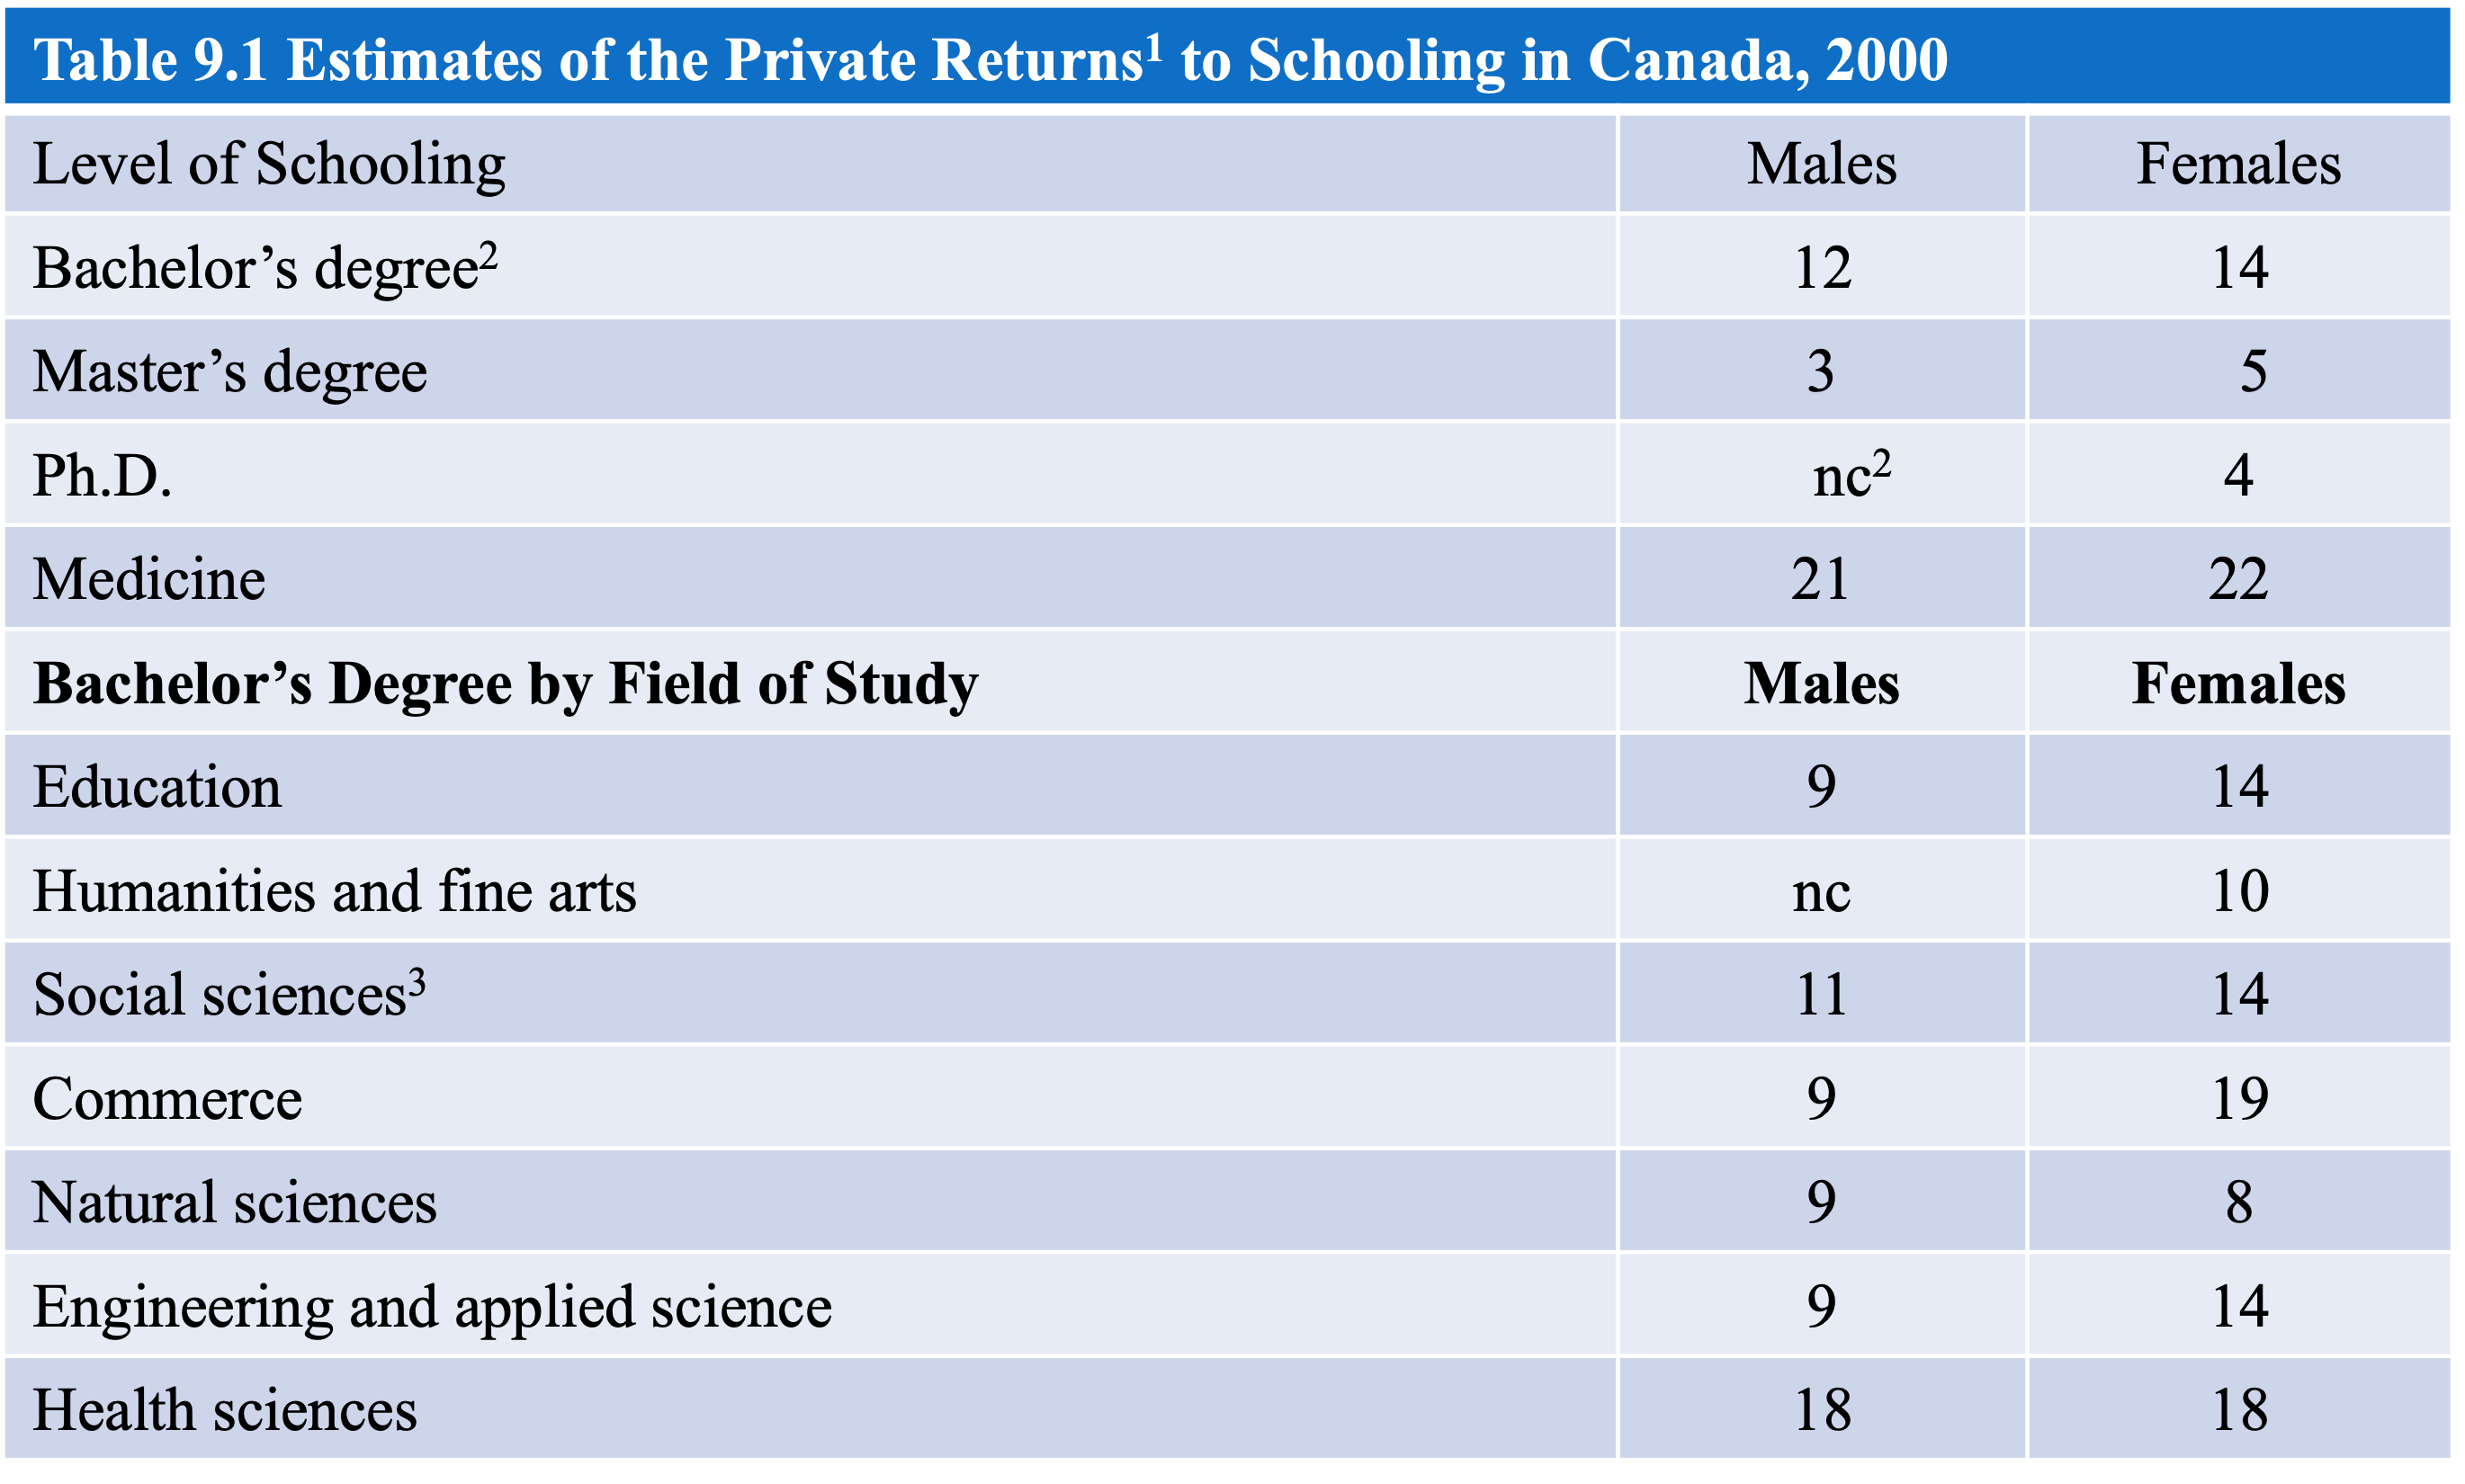
\includegraphics[width=0.8\linewidth]{T1}
\end{frame}

\begin{frame}{Reading Table 9.1}
\transfade
\begin{itemize}[<+->]
  \item Returns differ across:
  \begin{itemize}[<+->]
    \item level of schooling,
    \item gender,
    \item field of study.
  \end{itemize}
  \item Professional degrees such as medicine often have especially high returns.
  \item Returns to master's and PhD degrees are often smaller on the margin because those programs involve higher costs and longer time out of the labour market.
\end{itemize}
\end{frame}

\begin{frame}{Human Capital Earnings Function}
\transfade
A common empirical specification is:
\[
\ln Y = \alpha + rS + \beta_1 EXP + \beta_2 EXP^2 + \varepsilon
\]

where:
\begin{itemize}[<+->]
  \item \(Y\) = earnings,
  \item \(S\) = years of schooling,
  \item \(EXP\) = experience,
  \item \(r\) = estimated return to schooling.
\end{itemize}

\begin{block}{Interpretation}
The coefficient on schooling, \(r\), approximates the percentage increase in earnings from one additional year of education.
\end{block}
\end{frame}

\begin{frame}{Figure 9.5: Log Earnings by Years of Schooling}
\centering
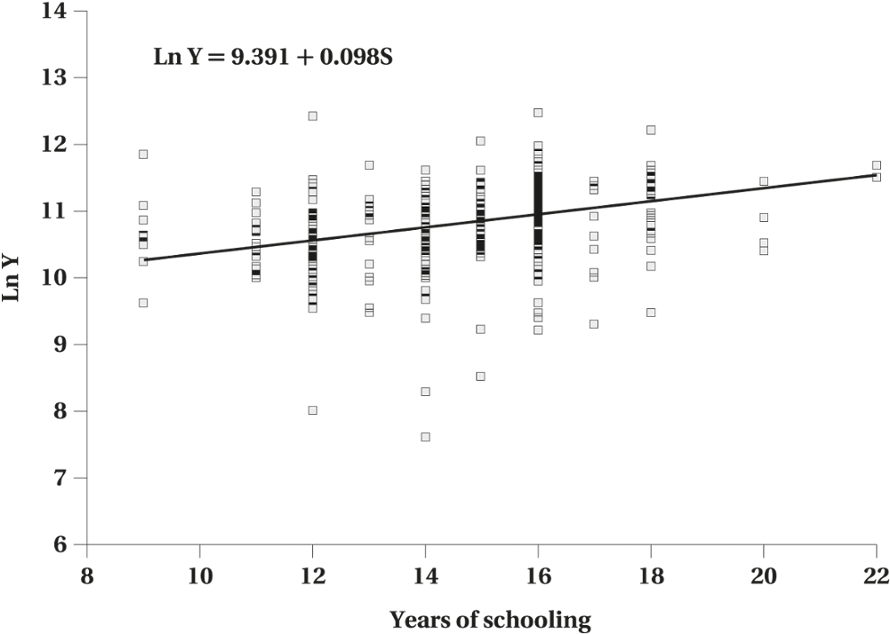
\includegraphics[width=0.6\linewidth]{F5}
\end{frame}

\begin{frame}{Table 9.2: Estimated Returns to Schooling and Experience}
\centering
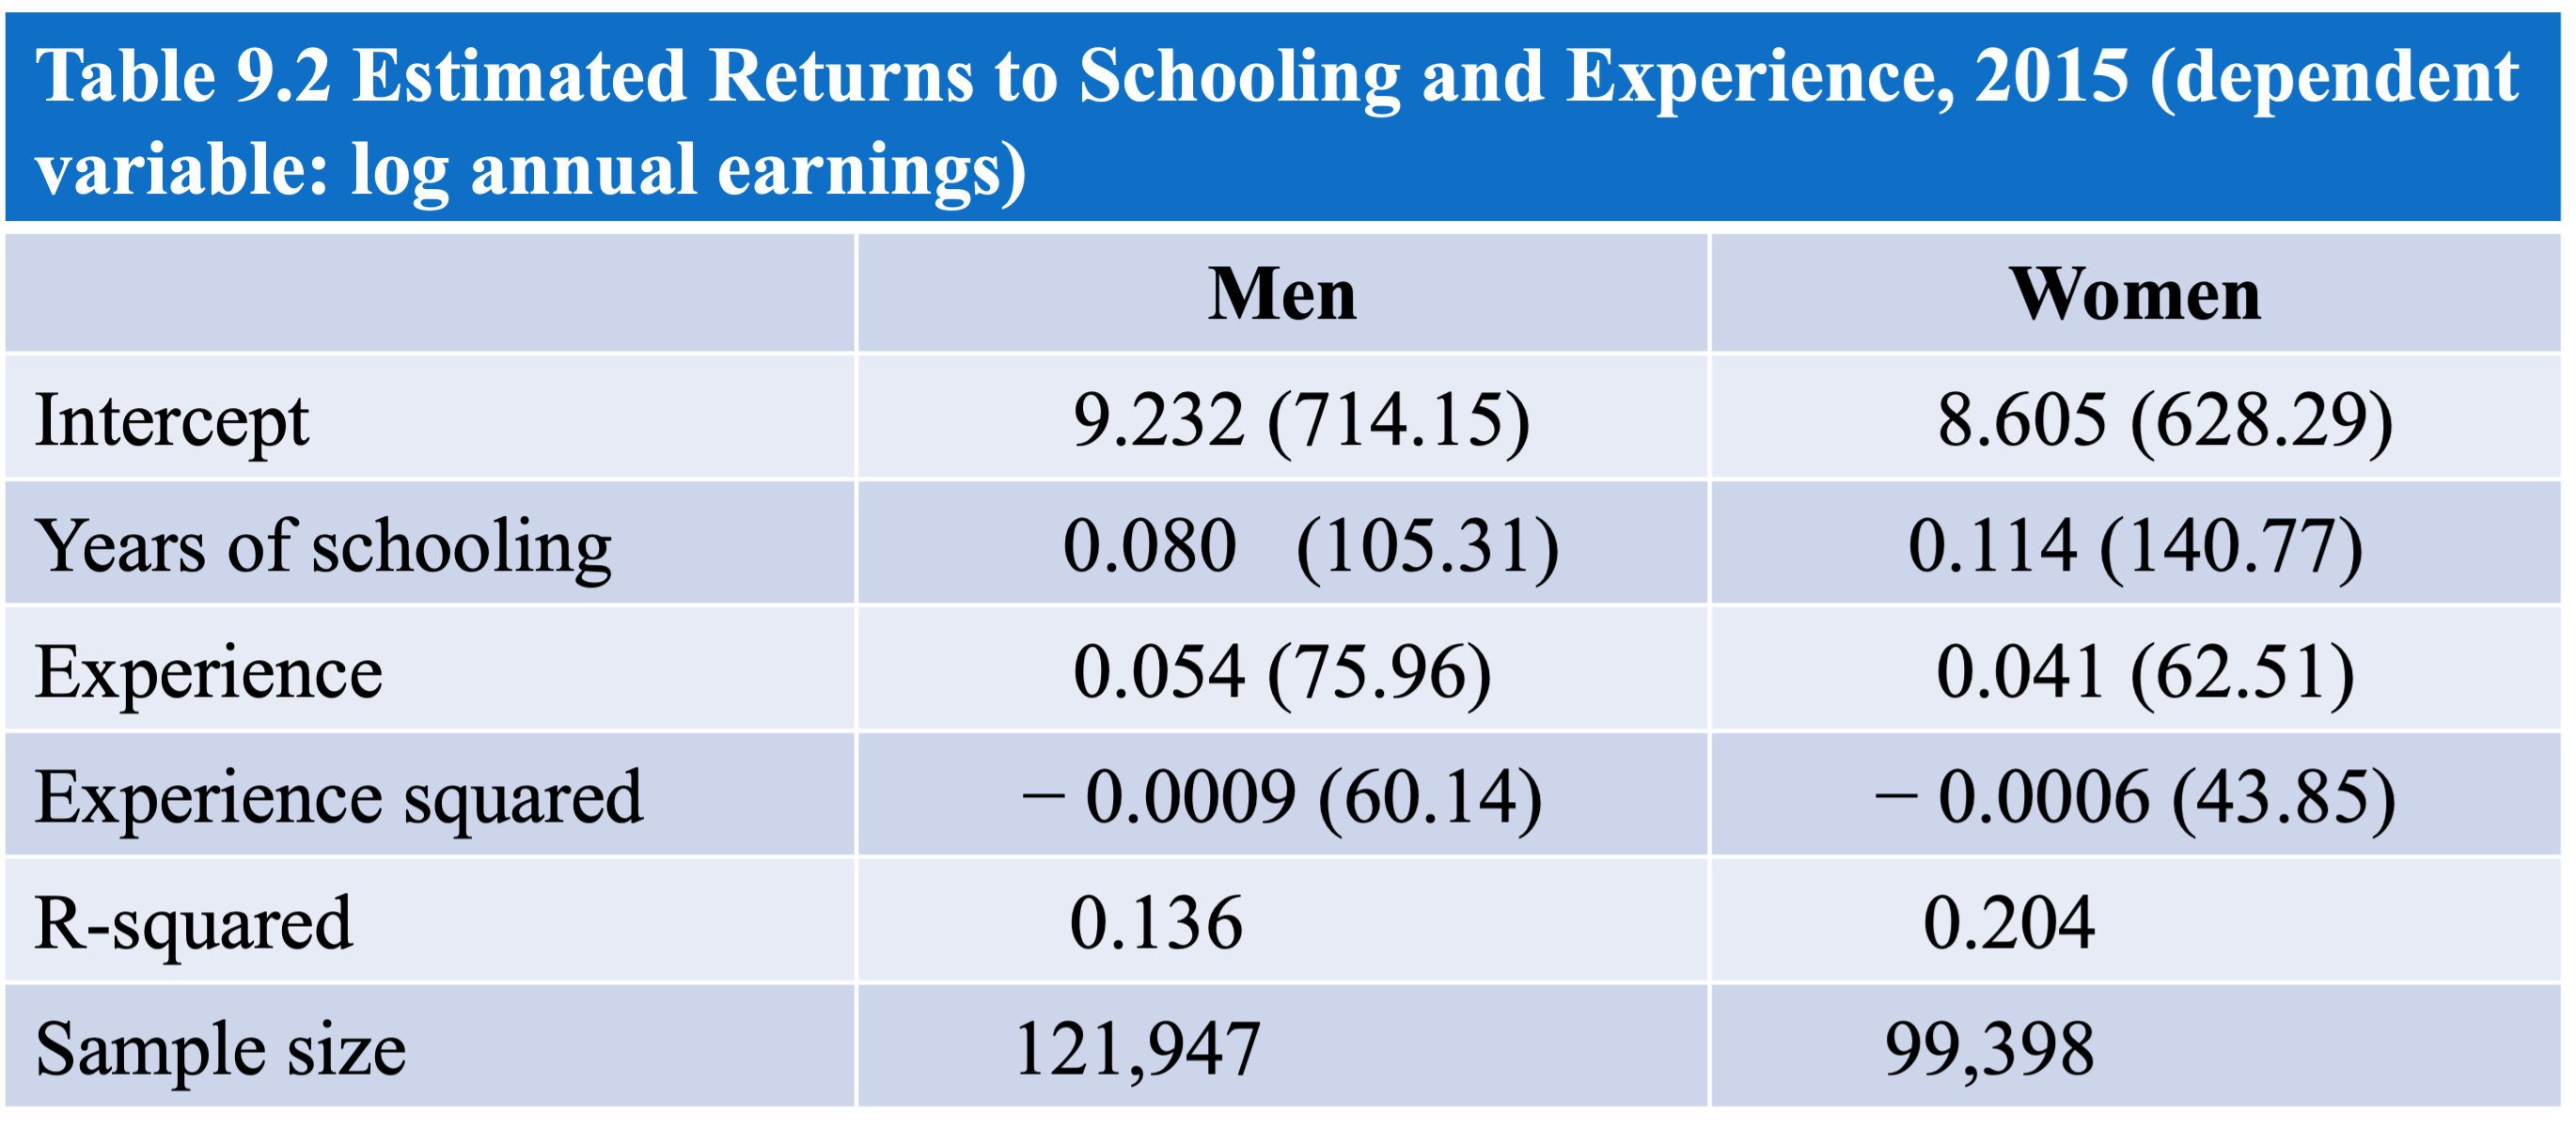
\includegraphics[width=0.9\linewidth]{T2}
\end{frame}

\begin{frame}{Interpreting the Earnings Function Results}
\transfade
\begin{itemize}[<+->]
  \item The schooling coefficient is positive for both men and women.
  \item Experience raises earnings, but at a decreasing rate:
  \begin{itemize}[<+->]
    \item positive coefficient on experience,
    \item negative coefficient on experience squared.
  \end{itemize}
  \item This produces the familiar concave age-earnings profile.
\end{itemize}
\end{frame}

% ============================================================
\section{Ability Bias, Signalling, and Social Returns}
% ============================================================

\begin{frame}{Empirical Evidence: Signalling, Screening, and Ability}
\transfade
\begin{itemize}[<+->]
  \item It is difficult to control for:
  \begin{itemize}[<+->]
    \item innate ability,
    \item motivation,
    \item perseverance,
    \item tolerance for effort.
  \end{itemize}
  \item These factors can bias estimated returns to education.
  \item This is known as \textbf{ability bias}.
\end{itemize}
\end{frame}

\begin{frame}{Addressing Ability Bias}
\transfade
Economists use several strategies:
\begin{itemize}[<+->]
  \item \textbf{Natural experiments}
  \item \textbf{Twin studies}
  \item \textbf{Compulsory school attendance laws}
  \item \textbf{Proximity to college} as an instrument for schooling
\end{itemize}

\begin{block}{Goal}
These methods try to separate the effect of education from unobserved ability.
\end{block}
\end{frame}

\begin{frame}{What Does the Evidence Suggest?}
\transfade
\begin{itemize}[<+->]
  \item The initial belief that returns to education were greatly overstated by ability bias appears to have been exaggerated.
  \item Education still seems to have a substantial causal effect on earnings.
  \item The measured returns discussed are usually \textbf{private monetary returns}.
\end{itemize}

\begin{block}{Important Distinction}
Private returns and social returns need not be the same.
\end{block}
\end{frame}

\begin{frame}{Social Returns to Education}
\transfade
\begin{itemize}[<+->]
  \item Social returns capture benefits beyond the individual's higher wages.
  \item Education may improve:
  \begin{itemize}[<+->]
    \item civic participation,
    \item health,
    \item lower crime,
    \item innovation,
    \item productivity spillovers.
  \end{itemize}
  \item Natural experiments based on regional differences in education are often used to estimate social returns.
\end{itemize}
\end{frame}

% ============================================================
\section{Returns to Education and Inequality}
% ============================================================

\begin{frame}{Increased Returns to Education and Inequality}
\transfade
\begin{itemize}[<+->]
  \item Increases in the return to education have occurred alongside broader increases in income inequality.
  \item However, the link is not complete.
  \item Inequality also depends on:
  \begin{itemize}[<+->]
    \item unemployment risk,
    \item within-group wage dispersion,
    \item top-end earnings growth.
  \end{itemize}
\end{itemize}
\end{frame}

\begin{frame}{Increasing Returns to Education Since 1980}
\transfade
\begin{itemize}[<+->]
  \item There was little change in returns to schooling in the 1980s and early 1990s.
  \item Returns increased substantially after the mid-1990s.
  \item Demand-side factors appear important:
  \begin{itemize}[<+->]
    \item skill-biased technological change,
    \item globalization,
    \item changing occupational structure.
  \end{itemize}
  \item Wage polarization and very high top incomes also matter.
\end{itemize}
\end{frame}

% ============================================================
\section{Training}
% ============================================================

\begin{frame}{Training}
\transfade
\begin{block}{Definition}
\textbf{Training} is an investment in skills acquired after labour market entry.
\end{block}
\begin{itemize}[<+->]
  \item \textbf{General training:} useful in many firms.
  \item \textbf{Specific training:} useful mainly in the firm providing the training.
\end{itemize}
\end{frame}

\begin{frame}{General Training}
\transfade
\begin{itemize}[<+->]
  \item Skills are transferable across firms.
  \item Other firms are willing to pay more for workers with these skills.
  \item Therefore workers are usually willing to bear much of the cost.
\end{itemize}

\begin{exampleblock}{Example}
Learning general software, accounting, or coding skills often raises wages across many employers.
\end{exampleblock}
\end{frame}

\begin{frame}{Specific Training}
\transfade
\begin{itemize}[<+->]
  \item Skills are valuable mainly to the current employer.
  \item Other firms will not pay a premium for these skills.
  \item Therefore the firm often pays at least part of the training cost.
\end{itemize}

\begin{exampleblock}{Example}
Training on a firm's proprietary software or internal production process is often specific training.
\end{exampleblock}
\end{frame}

\begin{frame}{Figure 9.6: Costs, Benefits, and Financing of Training}
\centering
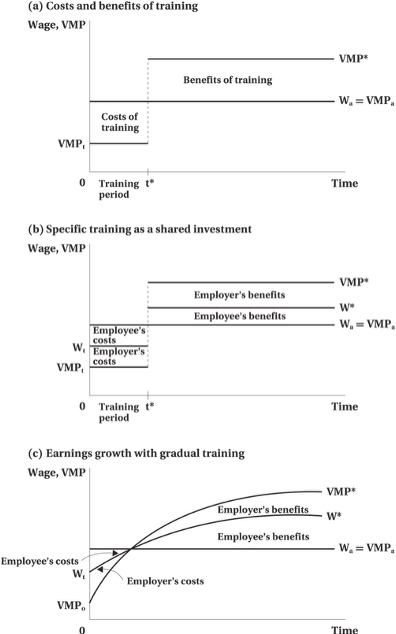
\includegraphics[width=0.3\linewidth]{F6}
\end{frame}

\begin{frame}{Who Should Pay for Training?}
\transfade
\begin{itemize}[<+->]
  \item \textbf{General training:} workers usually pay, often through lower trainee wages.
  \item \textbf{Specific training:} firms often pay, because the productivity gains are tied to that firm.
  \item In practice, costs may be shared when both parties benefit.
\end{itemize}
\end{frame}

\begin{frame}{Training and the Role of Government}
\transfade
\begin{itemize}[<+->]
  \item Private markets may provide less than the socially optimal amount of training because of:
  \begin{itemize}[<+->]
    \item imperfect information,
    \item regulatory restrictions,
    \item borrowing constraints,
    \item labour market disadvantage.
  \end{itemize}
  \item Training subsidies targeted to disadvantaged workers may:
  \begin{itemize}[<+->]
    \item increase working hours,
    \item raise wages,
    \item reduce poverty.
  \end{itemize}
\end{itemize}
\end{frame}

% ============================================================
\section{Chapter Summary}
% ============================================================

\begin{frame}{Chapter Summary}
\transfade
\begin{itemize}[<+->]
  \item Education and training are investments in \textbf{human capital}.
  \item The schooling decision compares present costs with future earnings benefits.
  \item The opportunity cost of time is often the largest cost of education.
  \item Human capital theory and signalling theory offer different explanations for the education--earnings link.
  \item Empirical evidence suggests that returns to education are substantial, though estimation must address ability bias.
  \item General and specific training differ in who should pay for them.
  \item Government may play a role when private markets underinvest in human capital.
\end{itemize}
\end{frame}

\begin{frame}
\centering
\Huge{\textbf{Thank You!}}
\end{frame}

\end{document}